\uuid{gIxq}
\exo7id{5521}
\titre{exo7 5521}
\auteur{rouget}
\organisation{exo7}
\datecreate{2010-07-15}
\isIndication{false}
\isCorrection{true}
\chapitre{Géométrie affine dans le plan et dans l'espace}
\sousChapitre{Géométrie affine dans le plan et dans l'espace}
\module{Géométrie}
\niveau{L2}
\difficulte{}

\contenu{
\texte{
Déterminer les différents angles d'un tétraèdre régulier (entre deux faces, entre deux arêtes et entre une arête et une face).
}
\reponse{
$$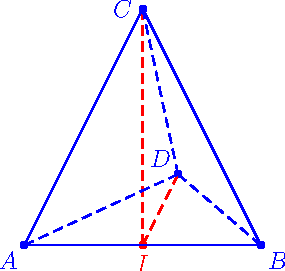
\includegraphics{../images/gIxq-1}$$


\textbf{Angle entre deux arêtes.} Les faces du tétraèdre $ABCD$ sont des triangles équilatéraux et donc l'angle entre deux arêtes est $60^\circ$.

$$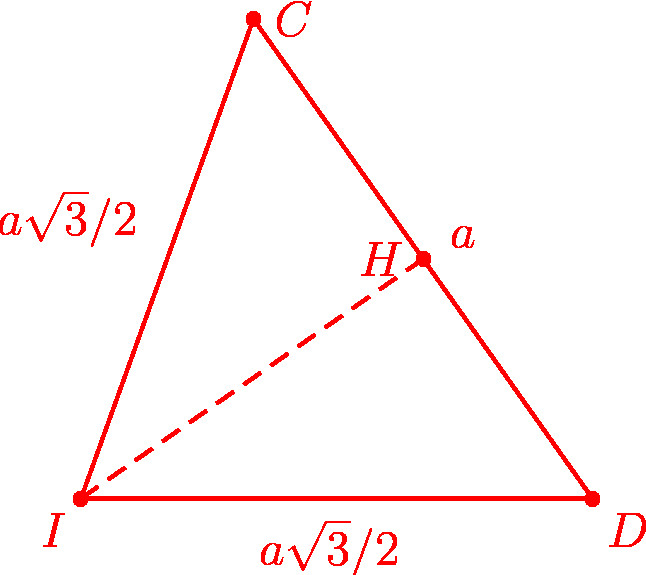
\includegraphics{../images/gIxq-2}$$

\textbf{Angle entre une  arête et une face.} C'est l'angle $\widehat{CDI}$ de la figure ci-dessus.

\begin{center}
$\widehat{CDI}=\Arccos\left(\frac{HD}{DI}\right)=\Arccos\left(\frac{a/2}{a\sqrt{3}/2}\right)=\Arccos\left(\frac{1}{\sqrt{3}}\right)=54,7\ldots^\circ$.
\end{center}
\textbf{Angle entre deux faces.} C'est l'angle $\widehat{CID}$ de la figure ci-dessus.

\begin{center}
$\widehat{CID}=\pi-2\widehat{CDI}=2\left(\frac{\pi}{2}-\Arccos\left(\frac{1}{\sqrt{3}}\right)\right)=2\Arcsin\left(\frac{1}{\sqrt{3}}\right)=70,5\ldots^\circ$.
\end{center}
}
}
